\chapter{Příklady na procvičení}
\subsection*{Příklad 1}
Je dána křivka
$$k(t) = [3\cos^3{t}, 3\sin^3{t}], t \in \langle0, 2\pi\rangle.$$
Napište souřadnice singulárních bodů. Pokud tyto body leží na jedné kružnici, napište její
parametrické vyjádření. \\
Napište souřadnice průsečíků křivky \textit{k} a přímek $y=x$ a $y=-x$. Napište obecné
rovnice tečen křivky v těchto průsečících. Křivku nakreslete.
\subsection*{Příklad 2}
Je dána křivka
$$k(t) = [3\cos{t}-\cos{3t}, 3\sin{t}-\sin{3t}], t \in \langle0; 2\pi\rangle.$$	
Napište souřadnice průsečíků křivky \textit{k} se souřadnicovými osami. Napište obecné rovnice
tečen v těchto průsečících. \\
Křivku nakreslete.	
\subsection*{Příklad 3}
Napište parametrické vyjádření 1 závitu ($t \in \langle0; 2\pi\rangle$) šroubovice bodu $A=[-3,4,5]$.
Osa levotočivého šroubového pohybu je osa \textit{z}. Redukovaná výška $v_0=2$. \\
Popište tečnu šroubovice v bodě $T=k\left(\frac{\pi}{2}\right)$ a napište obecnou rovnici normálové
roviny křivky v tomto bodě.
\subsection*{Příklad 4}
Je dána křivka
$$k(t) = [t^2+2t, -3t, t^3-t], t \in \mathbb{R}.$$
Popište tečny křivky, které jsou rovnoběžné s rovinou $\alpha: 2y+3z=0$.
\clearpage
\section{Výsledky}
\subsection*{Příklad 1}
\begin{figure}[H]
	\centering
	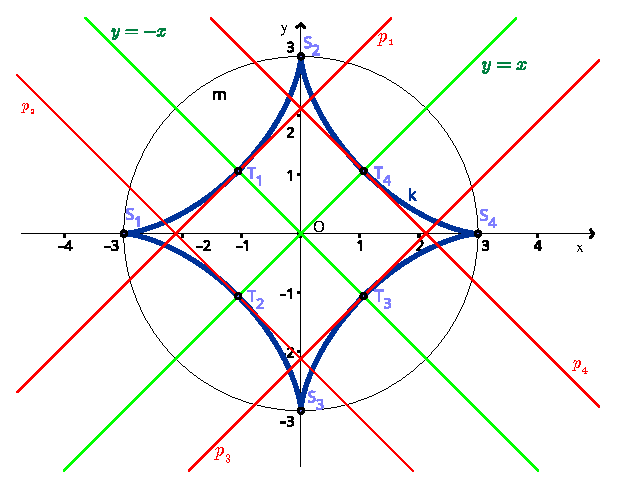
\includegraphics[height=330pt]{sam1.eps}
	\caption{Křivka \textit{k} pro $t \in \langle0, 2\pi\rangle$}
\end{figure} 
Křivka se nazývá \textit{astroida}. \\
Singulární body jsou
\begin{align*}
	S_1 & = k\left(\pi\right) = [-3, 0],                   \\
	S_2 & = k\left(\frac{\pi}{2}\right) = [0, 3],          \\
	S_3 & = k\left(\frac{3\pi}{2}\right) = [0, -3],        \\
	S_4 & = k\left(0\right) = k\left(2\pi\right) = [3, 0]. 
\end{align*}
Kružnice procházející singulárními body je
$$m(s) = [3\cos{t}, 3\sin{t}], s \in \langle0, 2\pi\rangle.$$
Průsečíky přímek $y=x$ a $y=-x$ s křivkou \textit{k} jsou
\begin{align*}
	T_1 & = \left[-\frac{3\sqrt{2}}{4}, \frac{3\sqrt{2}}{4}\right] = k\left(\frac{3\pi}{4}\right),  \\
	T_2 & = \left[-\frac{3\sqrt{2}}{4}, -\frac{3\sqrt{2}}{4}\right] = k\left(\frac{5\pi}{4}\right), \\
	T_3 & = \left[\frac{3\sqrt{2}}{4}, -\frac{3\sqrt{2}}{4}\right] = k\left(\frac{7\pi}{4}\right),  \\
	T_4 & = \left[\frac{3\sqrt{2}}{4}, \frac{3\sqrt{2}}{4}\right] = k\left(\frac{\pi}{4}\right).    
\end{align*}
Rovnice tečen v těchto bodech jsou
\begin{align*}
	p_1 & : x - y + \frac{3\sqrt{2}}{2} = 0, \\
	p_2 & : x + y + \frac{3\sqrt{2}}{2} = 0, \\
	p_3 & : x - y - \frac{3\sqrt{2}}{2} = 0, \\
	p_4 & : x + y - \frac{3\sqrt{2}}{2} = 0. 
\end{align*} 
\clearpage	  
\subsection*{Příklad 2}
\begin{figure}[H]
	\centering
	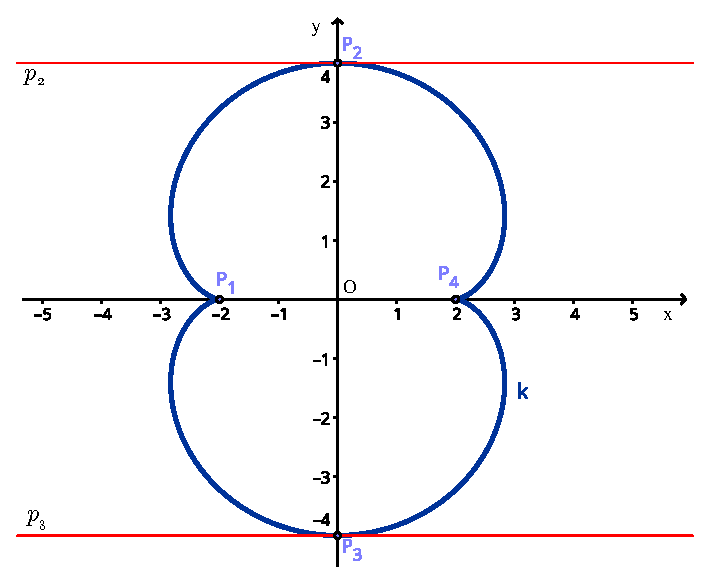
\includegraphics[height=330pt]{sam2.eps}
	\caption{Křivka \textit{k} pro $t \in \langle0, 2\pi\rangle$}
	
\end{figure} 
Průsečíky křivky \textit{k} se souřadnicovými osami jsou
\begin{align*}
	P_1 & = k(\pi) = [-2, 0],                       \\
	P_2 & = k\left(\frac{\pi}{2}\right) = [0, 4],   \\
	P_3 & = k\left(\frac{3\pi}{2}\right) = [0, -4], \\
	P_4 & = k(0) = k(2\pi) = [2, 0].                
\end{align*}
Body $P_1$ a $P_4$ jsou singulární body, neboť $k'(0)=k'(\pi)=k'(2\pi)=(0,0)$. \\
Tečny v bodech $P_2$ a $P_3$ jsou
\begin{align*}
	p_2: y & = 4  \\
	p_3: y & = -4 
\end{align*}  	
\clearpage
\subsection*{Příklad 3}	
\begin{figure}[H]
	\centering
	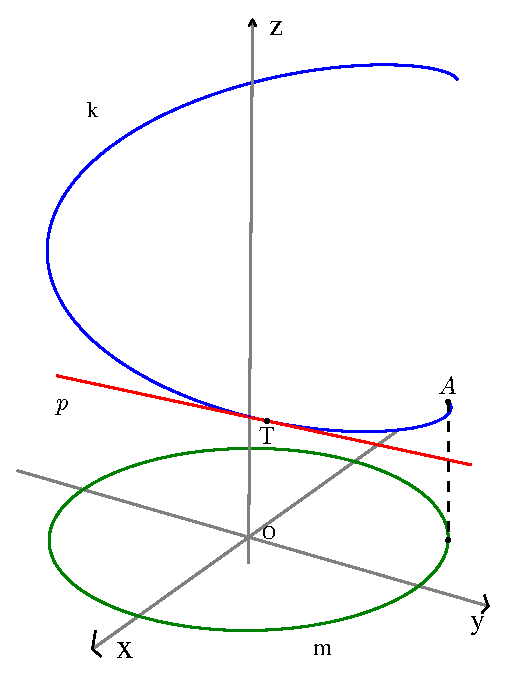
\includegraphics[height=330pt]{sam3.eps}
	\caption{Levotočivá šroubovice pro $t \in \langle0, 2\pi\rangle$}
	
\end{figure} 
Parametrické vyjádření jednoho závitu šroubovice \textit{k} je
$$k(t)=[-3\cos{t}+4\sin{t}, 4\cos{t}+3\sin{t}, 5+2t], t \in \langle0, 2\pi\rangle.$$
Tečna v bodě $T=k\left(\frac{\pi}{2}\right)=[4,3,5+\pi]$ je
$$p(s)=[4+3s, 3-4s, 5+\pi+2s], s \in \mathbb{R}.$$
Normálová rovina v bodě \textit{T} je
$$\alpha: 3x-4y+2z-10-2\pi=0.$$
\subsection*{Příklad 4}	
\begin{figure}[H]
	\centering
	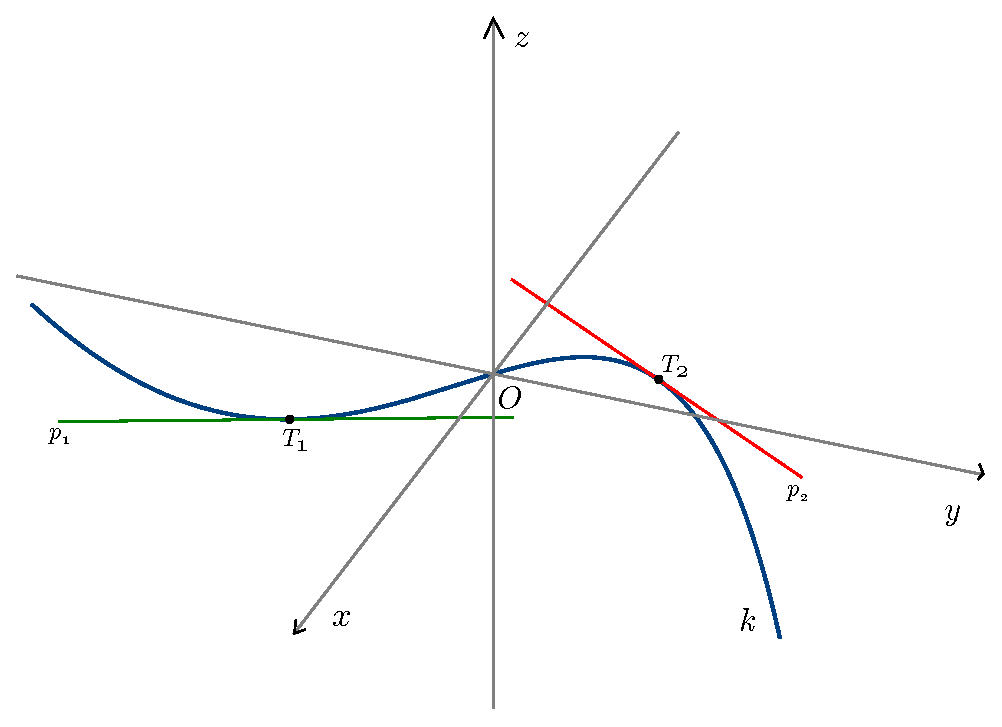
\includegraphics[height=300pt]{sam4b.eps}
	\caption{Křivka \textit{k} pro $t \in \langle-10, 10\rangle$}
	
\end{figure} 
Tečné vektory křivky \textit{k} jsou
$$k'(t)=(2t+2,-3,3t^2-1).$$
a vektor kolmý k $\alpha$ je $(0,2,3)$. \\
Aby byla tečna rovnoběžná s rovinou $\alpha$, musí být
$$(2t+2,-3,3t^2-1) \cdot (0,2,3)=0,$$
\begin{center}
	tj. $-6+9t^2-3=0$. \\
\end{center}
Tato rovnice má 2 řešení $t=1$ a $t=-1$. \\
Tečna v bodě $T_1=k(1)=[3,-3,0]$ je 
$$p_1(s)=k(1)+s \cdot k'(1), \quad p_1(s)=[3+4s,-3-3s, 2s], s \in \mathbb{R}.$$
Tečna v bodě $T_2=k(-1)=[-1,3,0]$ je 
$$p_2(u)=k(-1)+u \cdot k'(-1), \quad p_2(u)=[-1,3-3u, 2u], u \in \mathbb{R}.$$